% Drawing 154/02-25 -- folder 154, batch 02, archive page 37 (PDF page 38).
% Transcription: figure à gauche : un disque au bord vert traversé par deux cordes orange issues de deux points voisins du haut du bord, qui se rejoignent au bas ; le bord est prolongé au-dessous par un contour en pointillé où les deux cordes se croisent ; deux petits arcs foncés, sur le bord et sur le pointillé
% Kind: disk with two chords crossing just outside. Method 2 (schematic redraw from the facsimile). Status: ok.
% Notes: Light green rim; the two orange chords bulge apart and reach the bottom of the rim at two near points, cross just below it (point computed) and end on the dashed light green contour that prolongs the disk; a short dark green arc on the rim between the two chords and another on the dashed contour below the crossing. Redrawn 2026-11-12 (issue 128): to check again.
% Coordinates: 1 unit = 1 mm = 1/100 of the crop width (bbox in page fractions: [0.59, 0.425, 0.69, 0.5]).
% Redrawn by Claude (claude-fable-5-2), issue #128, 2026-11-12; not checked by a human; not compiled (no TeX in the session).
% Rights: reproduces part of the work -- behind RENDER_TRANSCRIPTS, never published by itself.
\documentclass[tikz,border=3pt]{standalone}
\usepackage{amsmath,amssymb}
\usetikzlibrary{patterns,arrows.meta}
\tikzset{Or/.style={orange!90!black}, Lg/.style={green!60!black!70}, Dg/.style={green!45!black}, pencil/.style={black!45}, struck/.style={black!35}, mpt/.style={circle,draw,inner sep=1.3pt}, pt/.style={circle,fill,inner sep=0.9pt}, opt/.style={circle,draw,fill=white,inner sep=1.1pt}}
\begin{document}
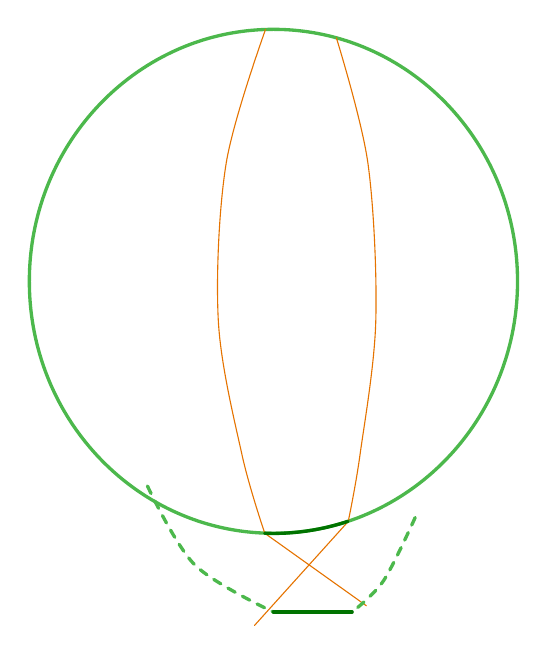
\begin{tikzpicture}[x=1mm,y=1mm,line cap=round,line join=round,font=\scriptsize]
\draw[Lg,very thick] (48,-50) ellipse[x radius=31, y radius=32];
\draw[Or] plot[smooth, tension=0.55] coordinates {(47,-18) (42,-35) (41,-55) (44,-72) (46.9,-82)};
\draw[Or] plot[smooth, tension=0.55] coordinates {(56,-19.1) (60,-35) (61,-55) (59,-72) (57.5,-80.5)};
\draw[Or] (46.9,-82) -- (59.8,-91.2);
\draw[Or] (57.5,-80.5) -- (45.6,-93.7);
\draw[Dg,very thick] (46.9,-82) arc[start angle=268, end angle=287.8, x radius=31, y radius=32];
\draw[Lg,dashed,very thick] plot[smooth, tension=0.55] coordinates {(32,-76) (38,-86) (48,-92)};
\draw[Lg,dashed,very thick] plot[smooth, tension=0.55] coordinates {(66,-80) (62,-88) (58,-92)};
\draw[Dg,very thick] (48,-92) -- (58,-92);
\end{tikzpicture}
\end{document}
